\documentclass[12pt]{article}
\usepackage[brazilian]{babel}
\usepackage[utf8]{inputenc}
\usepackage[T1]{fontenc}
\usepackage{float}
\usepackage{graphicx}

\graphicspath{{/home/matthias/Documents/reCastlevania/gdd/}}

\sloppy

\title{Entretenimento Digital \\ T1}

\author{Matthias Oliveira de Nunes}

\begin{document}

\maketitle

\begin{abstract}

Um jogo em que se pode explorar um mapa lutando contra vários monstros
poderosos. É um plataforma de ação com exploração.

\end{abstract}

\section{Tipo de jogo}

Um plataforma de ação em 2D.

\section{Descrição Geral}

Esse jogo foi inspirado na série $Castlevania$, tendo como personagem
controlável a Charlotte. O objetivo principal do jogo é eliminar todos os
inimigos, sendo essa a condição para passar para a próxima fase. A potuação é
baseada no número de inimigos mortos e no tempo gasto para passar de uma fase.

\section{Gameplay}

Os comandos do jogo serão feitos através do teclado. As teclas $WASD$
representam, respectivamente: para cima; para esquerda; para baixo; para
direita. A tecla $K$ representa o pulo enquanto a tecla $J$ o ataque. O $ESC$ é
usado para pausar/chamar o menu do jogo. As teclas $WASD$ também controlam o
menu do jogo, e nesse contexto, $K$ confirma enquanto $J$ cancela.

\section{Mapa do Ambiente}

\subsection{Fase 1}

\begin{figure}[H]
\centering
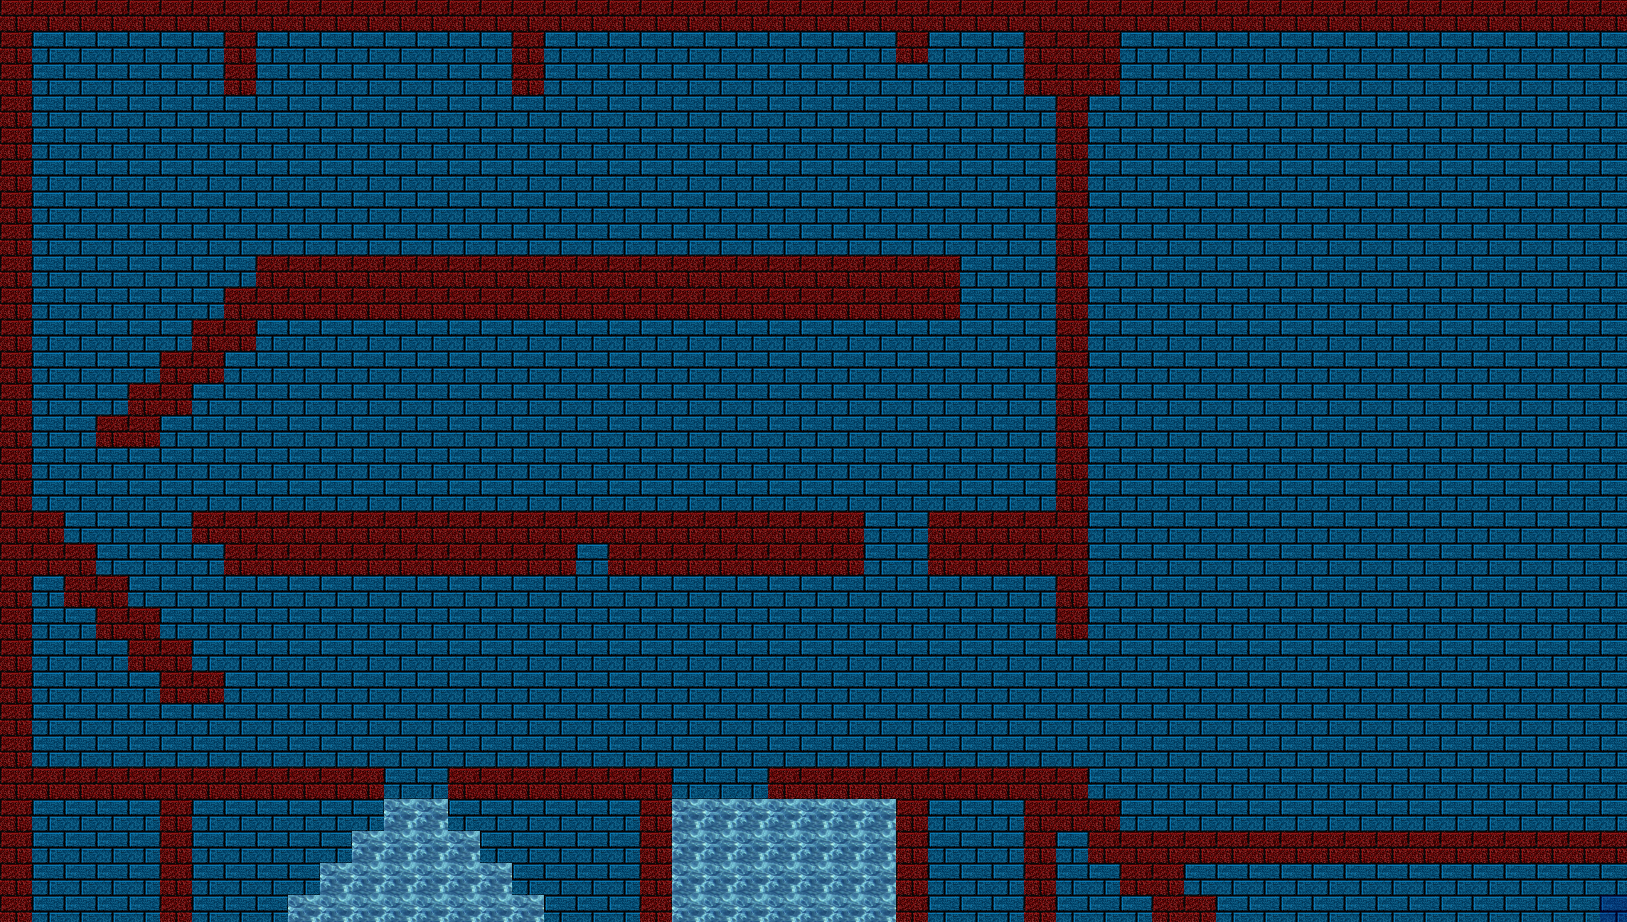
\includegraphics[width=100mm]{map1.png}
\caption{Fase 1}
\label{m1}
\end{figure}

Após matar todos os inimigos na fase 1, o jogador é levado à fase dois.

\subsection{Fase 2}

\begin{figure}[H]
\centering
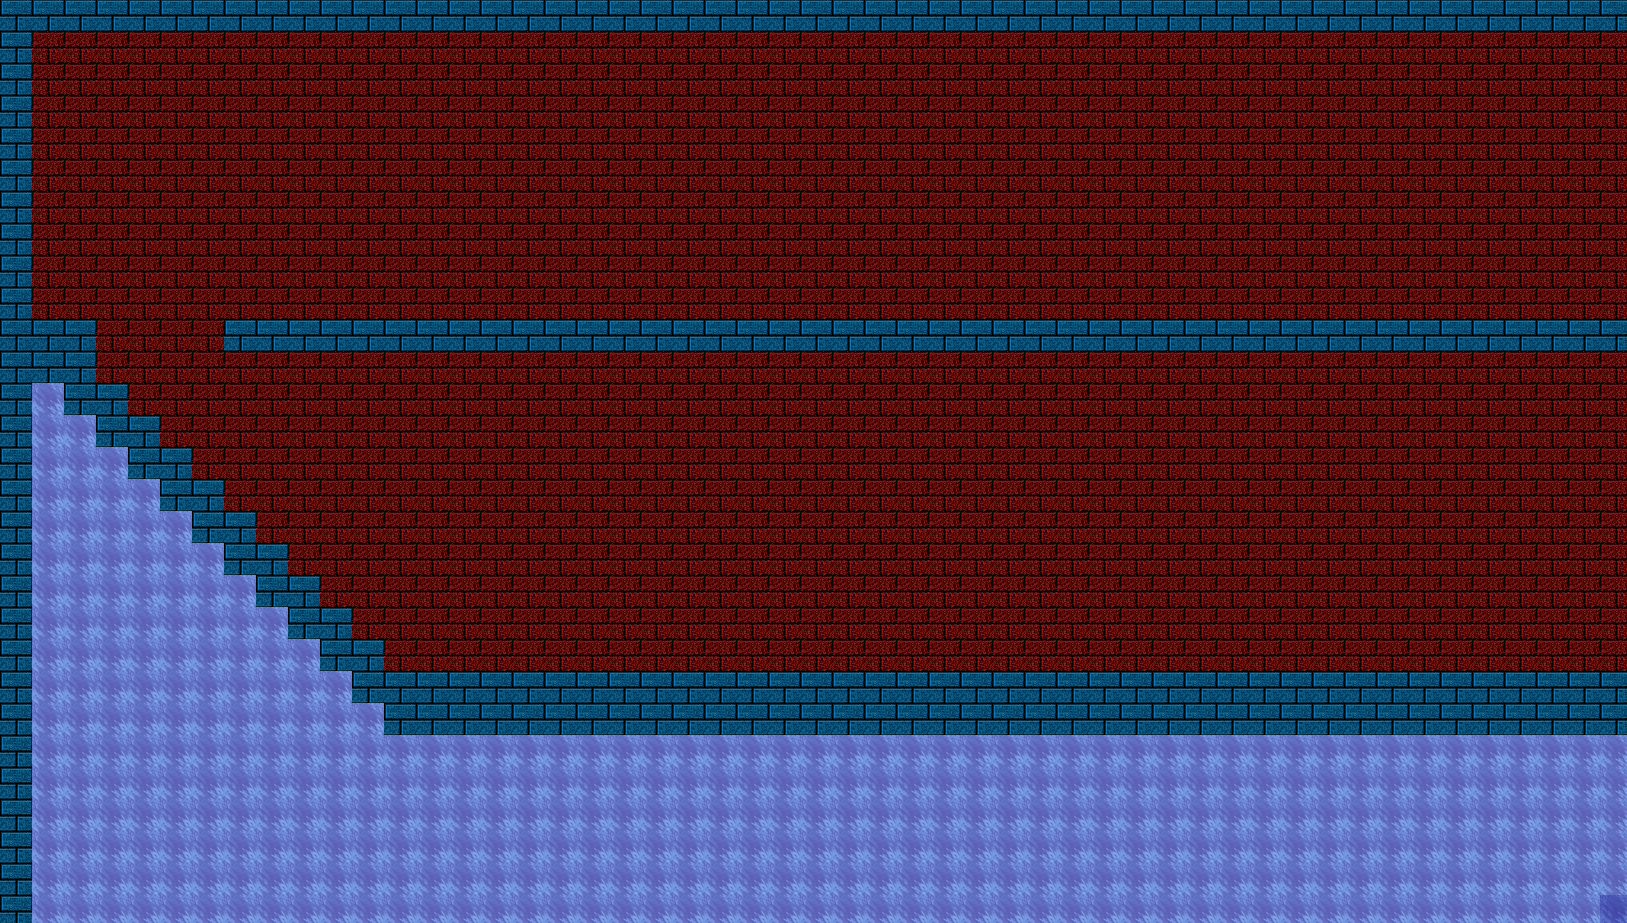
\includegraphics[width=100mm]{map2.png}
\caption{Fase 2}
\label{m2}
\end{figure}

Após matar todos os inimigos na fase 2, o jogador virou o jogo.

\section{Menus}

\subsection{Menu Principal}

\begin{figure}[H]
\centering
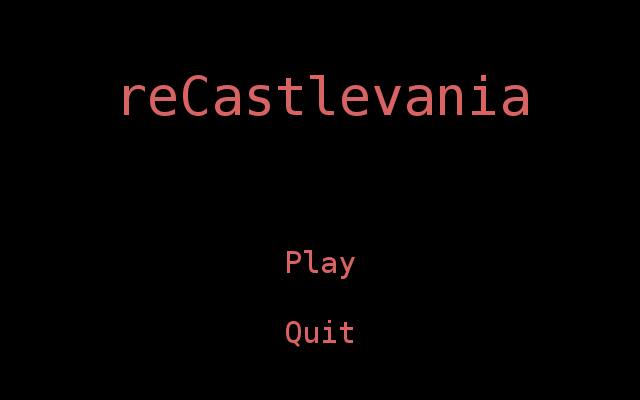
\includegraphics[width=100mm]{mainMenu.png}
\caption{Menu principal}
\label{mm}
\end{figure}

\subsection{Menu de Pausa}

\begin{figure}[H]
\centering
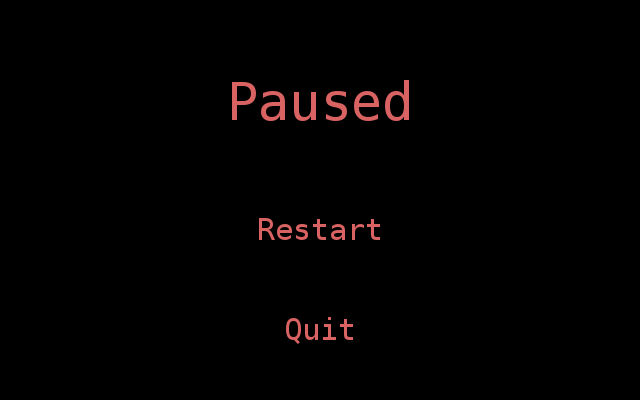
\includegraphics[width=100mm]{pauseMenu.png}
\caption{Menu de pausa}
\label{pm}
\end{figure}

\subsection{Tela de Pontuação}

\begin{figure}[H]
\centering
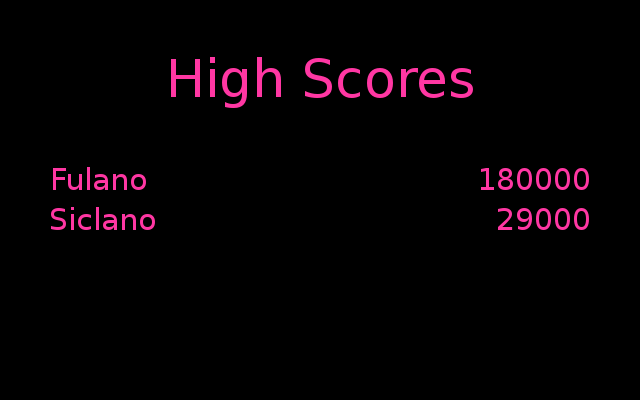
\includegraphics[width=100mm]{highScores.png}
\caption{Pontuação}
\label{hs}
\end{figure}

%\section{Requisitos de Audio}

%\section{Lista de Assets}

\end{document}
